\documentclass[12pt]{iopart}
\usepackage{iopams}
\usepackage{braket}
\usepackage{graphicx}
\usepackage{subfigure}
\usepackage{cite}
\usepackage{algorithm}
\usepackage{algorithmic}
%\usepackage{caption}
%\usepackage{subcaption}
%\usepackage{harvard}
%\usepackage{amsmath}
%\usepackage{amssymb}


\begin{document}
\newcommand{\swave}[0]{$\it{s}$-wave}
\newcommand{\pwave}[0]{$\it{p}$-wave}
\newcommand{\K}{$^{40}\rm{K}$}
\newcommand{\Rb}{$^{87}\rm{Rb}$}
\newcommand{\us}{$\rm{\mu s}$}
\newcommand{\mT}{$\rm{mT}$}
\newcommand{\ez}{$\bi{e_z}$}
\newcommand{\ex}{$\bi{e_x}$}
\newcommand{\um}{$\rm{\mu m}$}
\renewcommand{\thefootnote}{\arabic{footnote}}



\title[]{Direct observation of Feshbach enhanced \swave{} scattering of fermions}

\author{D Genkina$^1$, LM Aycock$^{1,2}$, BK Stuhl$^1$, H-I Lu$^1$ and IB Spielman
$^1$\footnote{Corresponding author}}

\address{$^1$Joint Quantum Institute, National Institute of Standards and Technology, and University of Maryland, Gaithersburg, MD, 20899 USA}
\address{$^2$Physics Department, Cornell University, Ithaca, NY 14850 USA}

\ead{ian.spielman@nist.gov}

\begin{abstract}
We directly measured the \swave{} scattering cross-section of ultracold \K{} atoms across the 20.2 \mT{} Feshbach resonance by colliding pairs of degenerate Fermi gases (DFGs) and imaging the scattered atoms.  We developed techniques to interpret absorption images in the regime where recoil induced detuning corrections are significant, and used those techniques to optimize the signal-to-noise ratio of atom number in scattering images. We extracted the scattered fraction for a range of bias magnetic field settings, and obtained a measurement of the Feshbach resonance's field location and width. These imaging techniques are generally applicable to experiments with lighter alkalis that would benefit from maximizing signal-to-noise ratio on the atom number counting at the expense of spatial imaging resolution.
\end{abstract}

\vspace{2pc}
\noindent{\it Keywords}: Quantum gases, Atomic physics

\maketitle

\section{Introduction}
Feshbach resonances are widely used for tuning the interaction strength in ultracold atomic gases. They have been particularly instrumental in the study of interactions and interaction-dependent processes in cold Fermi gases. In contrast to atomic Bose-Einstein condensates (BECs), where even weak interactions play a crucial role, for example giving rise to their characteristic Thomas-Fermi density profiles \cite{KetterleBEC},  interractions must compete with the Fermi energy before becoming relevant. Practically speaking, the density of Fermi clouds is typically $\sim$1000 times less than that of BECs \footnote{This is not the case for recently realized erbium and dysprosium DFGs \cite{Aikawa14,Lu12}, where strong dipolar interactions are present.}, making it necessary to enhance the strength of interactions in order to observe significant interaction effects\cite{KetterleDFG}. The tunability of interactions provided by Feshbach resonances has allowed for creation of molecular Bose-Einstein condensates from Fermi gases \cite{Greiner03,Zwierlein03, Jochim03} as well as observation of the phase transition from the Bardeen-Cooper-Schrieffer (BCS) superconduting regime to the BEC regime at sufficiently low temperatures \cite{Bartenstein04, Bourdel04, Zwierlein04, Regal04}.
\par A Feshbach resonance occurs when a diatomic molecular state energetically approaches the two-atom continuum \cite{Chin10, Timmermans99}. In experiment, the relative energy of the free atomic states in two hyperfine sublevels and the molecular state is defined by a bias magnetic field. Consequently, the Feshbach resonance can be accessed by changing the bias field. In the simple case where there are no inelastic two-body channels, such as for the \K{} resonance discussed in this work, the effect of the resonance on the scattering length between two free atoms is \cite{Chin10}
\begin{equation}
a(B)=a_{\rm{bg}}\left(1-\frac{\Delta}{B-B_0}\right),
\label{feshbachEq}
\end{equation}
where $a_{\rm{bg}}$ is the background scattering length, $\Delta$ is the width of the resonance, and $B_0$ is the field value at which the resonance occurs. The scattering length diverges at the resonance.
\par  The exact value of the resonant field $B_0$ is difficult to calculate analytically and is commonly computed via numerical models based on experimental input parameters \cite{Tiesinga93, Lysebo09, Gao11} or determined experimentally \cite{Inouye98, Cornish00}. Many experimental techniques have been used to characterize Feshbach resonances, including the observation of atom loss due to three-body inelastic scattering, measurement of re-thermalization timescales, and anisotropic expansion of the cloud upon release from a confining potential, all of which infer the elastic scattering cross section from collective behavior of the cloud \cite{Regal03,OHara02,Monroe93}.
\par Here we used direct scattering as a primary probe of the location and width of a Feshbach resonance. We collided pairs of ultra-cold Fermi gases and directly imaged the resulting \swave{} scattered atoms as a function of magnetic field strength. This allowed us to observe the enhancement in scattering without relying on proxy effects. We measured the fraction of atoms scattered during the collision, and from this fraction deduced the resonant magnetic field  and the width of the resonance.
%A similar technique has been used to characterize impurity scattering in BECs \cite{Chikkatur00}.
%\par The techniques developed in this experiment for observing Fermion scattering can be extended to engineering higher order partial wave interactions, as has been done for bosons \cite{Williams2012}.

In our dilute DFGs, even with the resonant enhancement of the scattering cross section, only a small fraction of the atoms scattered as the clouds passed through each other. This made direct detection of scattered atoms difficult due to detection uncertainty that disproportionately affected regions of low atomic density. To optimize the signal-to-noise ratio (SNR) for low atom numbers, we absorption imaged with fairly long, high-intensity pulses --- a non-standard regime, where the atoms acquired a velocity during imaging and the resulting Doppler-shift was non-negligible.  Simulation of the absorption imaging process was necessary for an accurate interpretation of these images. Using the simulation-corrected images, we extracted the fraction of atoms scattered in our collision experiment.

This paper is divided into two parts. In the first, we study absorption imaging in the presence of a significant time-dependent Doppler shift and show how we use our results to interpret data. In the second, we describe our \swave{} scattering experiment and extract a measure of the location and width of the Feshbach resonance in \K{}.

\section{Absorption imaging in the presence of strong recoil induced detuning}
\label{sec:2}
Absorption imaging measures the shadow cast by an atomic ensemble in an illuminating probe laser beam with angular frequency $\omega_{\rm{L}}$. This imaging technique relies on optical transitions between ground and excited atomic states. Such atomic transitions have an energy difference $\hbar\omega_0$, and a natural transition linewidth $\Gamma$. When interacting with a laser field an atom scatters photons from the laser field into the vacuum modes. In the two-level atom approximation, the rate of scattering is \cite{LCT}
\begin{equation}
\gamma_{\rm{sc}}= \frac{\Gamma}{2} \frac{\tilde{I}}{1+4\tilde{\delta}^2 +\tilde{I}},
\label{eq:scatrate}
\end{equation}
where $\tilde{I}=I/I_{\rm{sat}}$ is the laser intensity in units of the saturation intensity, and $\tilde{\delta}=\delta/\Gamma$ is the detuning $\delta=\omega_{\rm{L}}-\omega_0$ in units of the natural linewidth. 
\par An absorption image is obtained by shining an on- or near-resonant probe beam ($\tilde{\delta}\ll1$) onto the atomic cloud. Some of the light is scattered by the atoms, and the unscattered light, $\tilde{I}_f(x,y)$, is imaged onto a camera, as depicted in Fig. \ref{fig:absorptionIntor}(a) (top). The probe light is reapplied with the atoms absent to calibrate the intensity $\tilde{I}_0(x,y)$ of light unaffected by the atoms (bottom).
\begin{figure}
	\subfigure[]{\includegraphics*[scale=0.5]{Picture1a}}
	\subfigure[]{\includegraphics*{Picture1c.pdf}}
	\subfigure[]{\includegraphics*[scale=0.55]{Picture1b}}
\caption{Absorption imaging. (a) Near resonant probe light illuminates the atoms, and the transmitted light (containing a shadow of the atoms) is imaged on the camera. A second image taken with no atoms provides a reference. (b)  The probe beam is partially absorbed as it traverses the cloud, and the intensity seen by atoms further along the imaging direction \ez{} is lowered.  (c) An atomic cloud illuminated by a probe light field absorbs photons from the probe and re-emits them in all directions. This process results in a net acceleration of the cloud in the direction of the probe light as well as diffusive spreading in the transverse directions.  }
\label{fig:absorptionIntor}
\end{figure}

The intensity $\tilde{I}_f(x,y)$ is related to the number of atoms the light encountered. Consider the light as it travels along the imaging axis \ez{} through a 3D atomic density profile $\rho(x,y,z)$. We focus on a single pixel of the camera: sensitive to a single column of atoms $\rho(z)$ giving  $\tilde{I}_0$ and $\tilde{I}_f$. Our task is to invert the problem and obtain a column density $n = \int \rho\left(z\right) \,\mathrm{d}z$ given $\tilde{I}_0$ and $\tilde{I}_f$. As the light travels through a column of atoms, each atom scatters light according to Eq. (\ref{eq:scatrate}). Therefore, the atoms further along the imaging axis $z$ experience a reduced optical intensity due to attenuation of the laser field by the other atoms (Fig. \ref{fig:absorptionIntor}(b)). The intensity change from scattering as a function of $z$ is
\begin{equation}
\frac{d\tilde{I}(z)}{dz}=-\hbar\omega_{\rm{L}}\rho(z)\gamma_{sc}(z)=-\rho(z)\sigma_0\frac{\tilde{I}(z)}{1+4\tilde{\delta}^2 +\tilde{I}},
\label{eq:dIdz}
\end{equation}
where $\sigma_0$ is the resonant scattering cross section. Integrating this equation yields a relation between the observed optical depth $OD=-\ln \left(I_f/I_0\right)$ and the atomic column density $n$ \cite{Reinaudi07} --- we call the column density deduced in this manner $\sigma_0 n^{\rm{(1)}}$:
\begin{equation}
\sigma_0 n^{\rm{(1)}} = \left(1+4\tilde{\delta}^2\right)OD+ \tilde{I}_0-\tilde{I}_f.
\label{eq2}
\end{equation}
When the probe intensity is much smaller than the saturation intensity, $\tilde{I}_0\ll1$, and the probe light is on resonance, $\tilde{\delta}=0$, the right hand side of Eq. (\ref{eq2}) reduces to the optical depth \cite{Reinaudi07}, giving the simple relationship $\sigma_0 n^{\rm{(0)}}=OD$. 
\par Equations (\ref{eq:dIdz})-(\ref{eq2}) neglect the atomic recoil momentum and its effect on the laser detuning \cite{Konstantinidis12}. When an atom absorbs a photon from the laser light field it acquires a momentum kick $\hbar  k_{\rm{r}}$ in the direction of the light field. The associated recoil velocity is $v_{\rm{r}}=\hbar k_{\rm{r}}/m$, where $m$ is the atomic mass and $\hbar k_{\rm{r}}= h/\lambda$ is the recoil momentum from the laser with wavelength $\lambda$. Each re-emitted photon imparts a similar recoil momentum $\bi{p}_e$, but over many scattering events this momentum distribution averages to zero. Therefore the atom  will acquire an average velocity per photon $v_{\rm{r}}$ along \ez{}. The variance of $\bi{p}_e$, however, is not zero, allowing the atoms to acquire some momentum transverse to the laser field. While we ignore this correction, it results in the reduction of spatial resolution in the final image and its effect on the atomic cloud is pictured in Fig. \ref{fig:absorptionIntor}(c).
\par The average atom velocity parallel the light field after scattering $N$ photons is $N v_{\rm{r}}$ and it is Doppler shifted  $\delta= k_{\rm{r}} N v_{\rm{r}}$ from resonance. For any probe intensity, there is an imaging time that we call the recoil time $t_{\rm{r}}$ after which  $\delta>\Gamma/2$ and, even if the probe beam is initially on resonance with the atomic transition, we cannot neglect the detuning's  effect on the scattering rate. Furthermore, this detuning varies both with imaging time $t$ and with distance along the propagation direction $z$ (Fig. \ref{fig:expos}(a)). Thus, the laser's spatially varying intensity profile in the atomic cloud also depends on time:
\begin{equation}
\frac{d\tilde{I}(t,z)}{dz}=-\sigma_0 \rho(t,z) \frac{\tilde{I}(t,z)}{1+4\tilde{\delta}(t,z)^2 +\tilde{I}(t,z)}. \label{eq3}
\end{equation}
Assuming that the atoms do not move significantly during the imaging time (we will remove this assumption shortly), the dimensionless detuning is
\begin{equation}
\tilde{\delta}(t,z)=\frac{ k_{\rm{r}} v_{\rm{r}}}{2\sigma_0 \rho(t,z)}\int_0^t \frac{d\tilde{I}(z,\tau)}{dz}\,\mathrm{d}\tau; \label{eq4}
\end{equation}
the relationship between the atomic density and the observed intensities is no longer straightforward.
\begin{figure}
	\subfigure[]{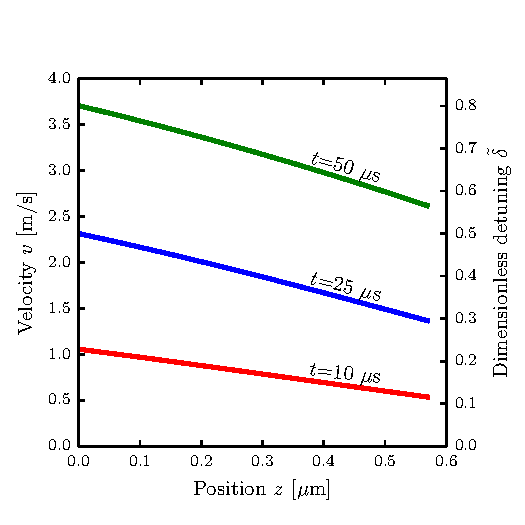
\includegraphics{figure1.pdf}}
	\subfigure[]{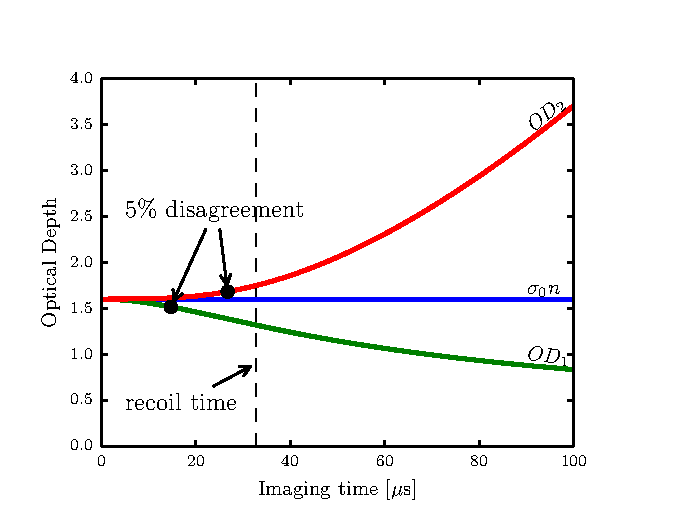
\includegraphics{figure2.pdf}}
\caption{(a) Dependence of velocity and detuning on position simulated for \K{} at three different imaging times and a probe intensity $\tilde{I}_0=0.8$. (b) Column densities deduced from optical depths obtained from recoil detuning corrected simulation of on-resonant imaging of $^{40}K$ atoms at probe intensity $\tilde{I}_0=0.8$. The input column density $\sigma_0 n=1.6$. $\sigma_0 n^{\rm{(1)}}$ is the high probe intensity corrected column density given by Eq. (\ref{eq2}). $\sigma_0 n^{\rm{(2)}}$ is the column density as expanded to second order in time, Eq. (\ref{eq:OD2}).}
\label{fig:expos}
\end{figure}
\par By considering this equation perturbatively in imaging time we obtain corrections to second order \cite{LJLthesis}

\begin{eqnarray}
&\sigma_0 n^{\rm{(2)}}  =  c_0+c_1t+c_2t^2, \mbox{ where } \\
 &c_0= \sigma_0 n^{\rm{(1)}}, c_1=0, c_2=\frac{( k_{\rm{r}} v_{\rm{r}})^2}{3}\left[\frac{1}{\tilde{I}_f+1}-\frac{1}{\tilde{I}_0+1}+\mathrm{ln}\left(\frac{\tilde{I}_f+1}{\tilde{I}_0+1}\right)\right]
\label{eq:OD2}
\end{eqnarray}
As shown in  Fig. \ref{fig:expos}(b), the perturbative treatment is accurate to times up to the recoil time after which it begins to diverge. To adequately correct for the recoil induced detuning of the atoms, we numerically simulated the imaging process to obtain $\tilde{I}_f$ as a function of imaging time, atomic density, and probe intensity.
%\begin{figure}
%	\includegraphics*{figure2.pdf}
%\caption{Using time dependent $I_f$ values obtained from recoil detuning corrected simulation of on-resonant imaging of $^{40}K$ atoms at probe intensity $I_0=0.8\, I_{\rm{sat}}$, this graph shows the optical depths obtained by each model. The `true' optical depth is $\sigma_0 n=1.6$. $OD_1$ is the high probe intensity corrected optical depth given by Eq. (\ref{eq2}). $OD_2$ is the high probe intensity corrected and expanded to second order in time optical depth, Eq. (\ref{eq:OD2}) \cite{LJLthesis}. The recoil time is the time it takes for the cloud, on average, to become detuned by a linewidth $\Gamma$. Both models start to differ from the true value before a recoil time.  }
%\label{fig:ODcorrections}
%\end{figure}
\par In the following, we describe two versions of this simulation. First, we took a simplistic approach where the spatial distribution of atoms did not change appreciably during the imaging time: $vt\ll I_0/(\hbar \omega_{\rm{L}} \gamma_{\rm{sc}} \rho)$. We verified this approach in known limits and then cross-checked the validity of the static assumption. For realistic input parameters, we found this assumption to be invalid. We then developed a quasi-classical approach and allowed the atoms to move during the imaging time. While the atomic trajectories were wildly different than in the static atom approximation, we found that the predicted $OD$s only differed on the 0.5$\%$ level.


\subsection{Stationary atom model}
To solve Eqs. (\ref{eq3})-(\ref{eq4}), we divided the cloud into spatial bins.  In this approximation, the number of atoms in each bin was time-independent.  The algorithm used is shown in Alg. (\ref{algorithm1}), in which we took a Gaussian profile for our initial density distribution. We call the optical depth simulated by this algorithm the simulated optical depth $OD^{\rm{sim1}}$.

\begin{algorithm}
\caption{Stationary atom model}
\label{algorithm1}
\begin{algorithmic}
\STATE $I[n=0,t]=I_0$ \COMMENT{$n$ is the bin index, $t$ is the time index, $I$ is in units of $I_{\rm{sat}}$}
\STATE $\delta[n, t=0]=0$ \COMMENT{light initially resonant, $\delta$ in units of $\Gamma/2$}
\STATE $H_f=0$ \COMMENT{Radiant fluence seen by camera after passing through cloud}
\FOR[loop over time steps]{$t=0$ to $t_f$}
 \FOR[loop over bins, N is total bin number]{$n=1$ to $N$}
 \STATE $A=\sigma_0\rho[n] dz$ \COMMENT{$dz$ is the size of spatial step}
 \STATE $B=v_{\rm{r}} dt/(\hbar c \rho[n])$  \COMMENT{$dt$ is the size of the time step}
\STATE $I[n,t]=I[n-1,t] - A I[n-1,t]/(1+\delta[n,t-1]^2+I[n-1,t])$  \COMMENT{Eq. (\ref{eq3})}
\STATE $\delta[n,t]=\delta[n,t-1]+B\left(I[n-1,t]-I[n,t]\right)$  \COMMENT{Eq. (\ref{eq4})}
\ENDFOR
\STATE $H_f =H_f+ I[N,t]dt$ \COMMENT{collecting total fluence seen by the camera}
\ENDFOR
\STATE $OD^{\rm{sim1}}=-\ln{(H_f/I_0t_f)}$
\end{algorithmic}
\end{algorithm}

\par We checked the validity of our simulation in the limits where the problem is analytically solvable. In the limit where the probe intensity is much weaker than the saturation intensity, $\tilde{I}_0\ll 1$, the atoms' velocities are hardly changed, and Eq.(\ref{eq3}) reduces to
\begin{eqnarray}
\frac{d\tilde{I}(z)}{dz}&=-\rho\sigma_0\tilde{I}(z), \mbox{ from which we recover the analytic form }\\
\sigma_0 n^{\rm{(0)}} &= -\ln\tilde{I}_0/\tilde{I}_f. \label{eq6}
\end{eqnarray}
In the limit where the probe intensity is much larger than the saturation intensity, $\tilde{I}_0\gg \tilde{\delta}$, even far detuned atoms will scatter light at their maximum rate. The time dependence of the detuning can thus be neglected, and Eq. (\ref{eq3}) becomes
\begin{eqnarray}
\frac{d\tilde{I}(z)}{dz}&=-\rho\sigma_0, \mbox{ which integrates to }\\
\sigma_0 n &= \tilde{I}_0 - \tilde{I}_f. \label{eq8}
\end{eqnarray}
We recognize the right hand sides of Eq. (\ref{eq6}) and Eq. (\ref{eq8}) as the two terms in Eq. (\ref{eq2}). Thus, as shown in  Fig. \ref{fig:IsatLimits}, $OD^{\rm{sim1}}$  coincides with the optical depth as predicted by Eq. (\ref{eq2}) in both the small and large probe intensity limits.
\begin{figure}
	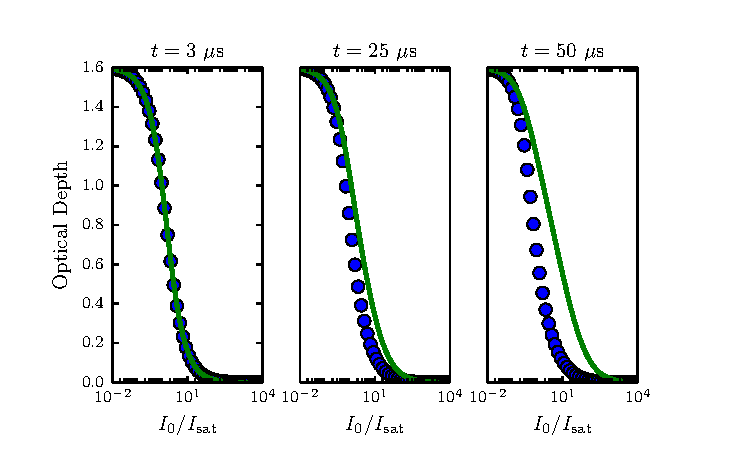
\includegraphics{figure3.pdf}
\caption{Optical depth as a function of probe intensity as predicted by the simulation (blue symbols) and by Eq. (\ref{eq2}) (green curves), for three different imaging times. As expected, the predictions agree in both the high and low intensity limits, and differ for probe intensities comparable to the saturation intensity and longer imaging times. }
\label{fig:IsatLimits}
\end{figure}
\par We used the results of this simulation to check the self-consistency of the  stationary atom assumption, i.e. the distance traveled by the atoms (as deduced from integrating the acquired recoil velocity over the imaging time) is less than the bin size. As can be seen from Fig. \ref{fig:simTests}(a), not only do the atoms travel more than the bin size, but they travel far beyond the initial extent of the cloud. Moreover, owing to the higher initial scatter rate, the back of the cloud overtakes the front for long imaging times. Thus, the atomic distribution as a function of position changes dramatically during the imaging pulse, and the stationary assumption is invalid.
\begin{figure}
	\subfigure[]{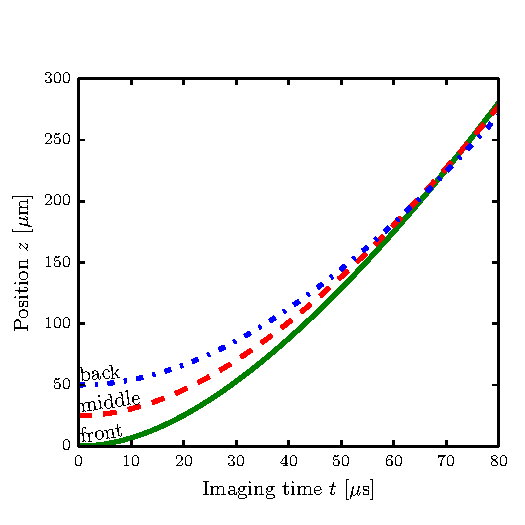
\includegraphics{figure4.pdf}}
	\subfigure[]{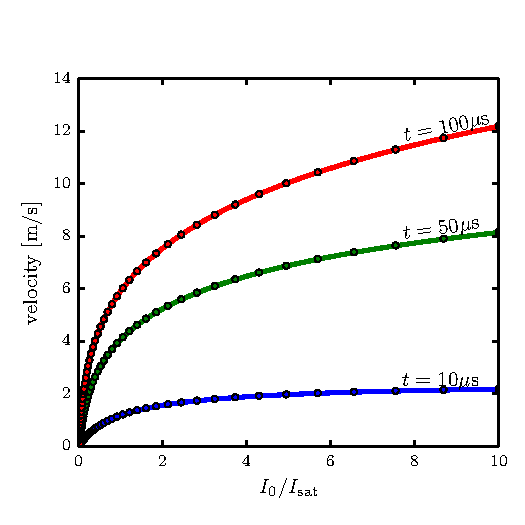
\includegraphics{figure5.pdf}}
\caption{(a) Position of atoms as a function of imaging time for atoms in the first (solid green), middle (dashed red), and last (dotted blue) bins of the simulated density distribution for an initial cloud 50 \um{} in extent. The probe intensity used in this calculation was $1.2\, I_{\rm{sat}}$, and the column density was $\sigma_0 n=1.6$. (b) The velocity of a single composite atom as a function of probe intensity for various imaging times. Simulation data (dots) and numerical  solutions of Eq. (\ref{eq10}) (lines) are in agreement.}
\label{fig:simTests}
\end{figure}

\subsection{Traveling atom model}
To account for the changing atomic distribution during the imaging pulse, we numerically simulated the classical kinetics of atoms subject to the recoil driven optical forces. To simulate large ensembles in a reasonable time, we modeled composite atoms, each describing the aggregate behavior of $N_{\rm{ca}}$ atoms. The amended algorithm is shown in Alg. (\ref{algorithm2}).
\begin{algorithm}
\caption{Travelling atom model}
\label{algorithm2}
\begin{algorithmic}
\STATE $z[n]=z_0$, $\delta[n]=0$ \COMMENT{initialize position and detuning for each composite atom, labeled by index $n$}
\STATE $O[i]=n$ \COMMENT{make a list of composite atom indexes, ordered by position}
\STATE $I[n=0,t]=I_0$ \COMMENT{ $t$ is the time index, $I$ is in units of $I_{\rm{sat}}$}
\STATE $H_f=0$ \COMMENT{Radiant fluence seen by camera after passing through cloud}
\FOR[loop over time steps]{$t=0$ to $t_f$}
 \FOR[loop over superatoms]{$i=1$ to $N$}
\STATE $n=O[i]$ \COMMENT{apply probe intensity to composite atoms in order of appearance}
 \STATE $A=\sigma_0 N_{sa} dz$ \COMMENT{dz is length over which atoms were grouped into single composite atom}
 \STATE $B=v_{\rm{r}} dt/(\hbar c  N_{sa})$  \COMMENT{dt is the time step}
\STATE $I[n,t]=I[n-1,t] - A I[n-1,t]/(1+\delta[n]^2+I[n-1,t])$  \COMMENT{Eq. (\ref{eq3})}
\STATE $\delta[n]\mathrel{+}=B\left(I[n-1,t]-I[n,t]\right)$  \COMMENT{Eq. (\ref{eq4}), detuning in units of $\Gamma/2$}
\STATE $z[n]\mathrel{+}=dt\Gamma\delta/2k$ \COMMENT{$k$ is the wavenumber, $\Gamma\delta/2k$ is the velocity at $\delta$ detuning}
\ENDFOR
\STATE $O[i]$=sort($n$, key =$z[n]$) \COMMENT{sort composite atom indexes by current position}
\STATE $H_f H_f+ I[N,t]dt$ \COMMENT{collecting total fluence seen by the camera}
\ENDFOR
\STATE $OD^{\rm{sim2}}=-\ln{(H_f/I_0t_f)}$
\end{algorithmic}
\end{algorithm}
\par To validate our code, we again checked the velocity predicted in this model against known limits. One such limit is that of a single composite atom. In this case, there is no attenuation, and the intensity seen by the composite atom is constant at $\tilde{I}_0$. Only the detuning  evolves in time, and Eqs. (\ref{eq3}) and (\ref{eq4}) give
\begin{equation}
\frac{d\tilde{\delta}(t)}{dt}= \frac{ k_{\rm{r}} v_{\rm{r}}}{2} \frac{\tilde{I}}{1+4\tilde{\delta}^2+\tilde{I}}.
\label{eq10}
\end{equation}
Equation (\ref{eq10}) can be solved numerically, and is in agreement with our simulation, as seen in Fig. \ref{fig:simTests}(b).
%\begin{figure}
%	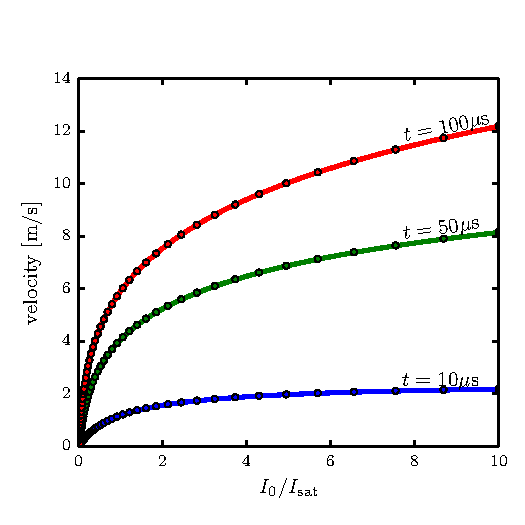
\includegraphics{figure5.pdf}
%\caption{The velocity of a single superatom as a function of probe intensity for various imaging times. Simulation data (dots) and numerical  solutions of Eq. (\ref{eq10}) (lines) are in good agreement.}
%\label{fig:oneAtomVel}
%\end{figure}
\par We used this model to study the time evolution of the cloud shape during imaging and visualized the phase space evolution of superatoms, shown in Fig. \ref{fig:phaseSpace}. The cloud is strongly distorted during imaging.
\begin{figure}
	\subfigure[]{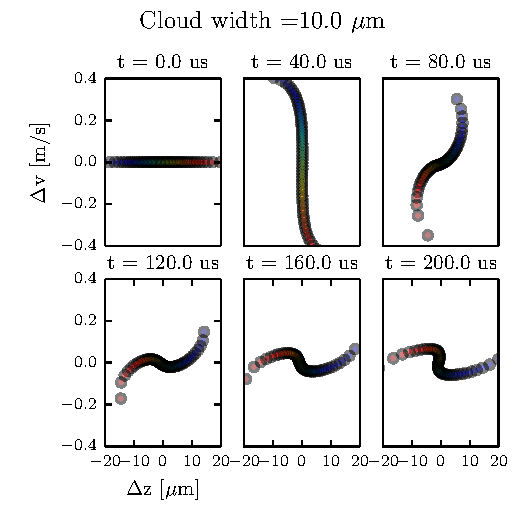
\includegraphics{figure6a.pdf}}
	\subfigure[]{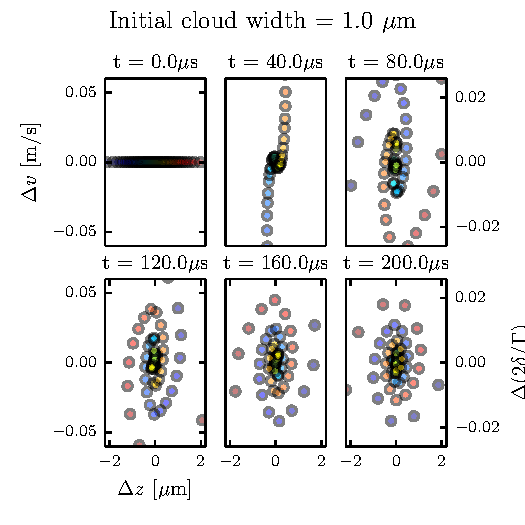
\includegraphics{figure6b.pdf}}
\caption{Phase space evolution of an atomic cloud exposed to probe light with intensity $\tilde{I}_0=1.2$. We defined $\Delta v=v -\left< v(t) \right>$  and $\Delta z=z-\left< z(t) \right>$, subtracting out the center of mass position and velocity of the cloud. The column density $\sigma_0 n$ is 1.6, and the initial cloud is a Gaussian with a width of 10 $\mu$m in (a) and 1 $\mu$m in (b). The center of mass velocities $\left< v\right>$ are (0,  3.41, 5.26, 6.52, 7.50, 8.32) m/s sequentially, and are the same for both initial cloud widths. }
\label{fig:phaseSpace}
\end{figure}
\par We compared the optical depths predicted by each of the two models, $OD^{\rm{sim1}}$ and $OD^{\rm{sim2}}$. As seen Fig. \ref{fig:compareModelsAndIsat}(a), the predicted optical depths were hardly changed by including the full time evolution:  $\left|OD^{\rm{sim1}}-OD^{\rm{sim2}}\right|/OD^{\rm{sim1}} \le 0.005$. Thus, for the purposes of deducing the atom density from experimental optical depths, the stationary atom model is sufficient. Furthermore, we simulated a range of initial density profiles $\rho(z)$, and found their impact to be negligible \--- the only observable is the integrated atomic density $n=\int\rho(z)\mathrm{d}z$. Still, for interpreting experimental images, we used the data generated by the traveling atom simulation.
\begin{figure}
	\subfigure[]{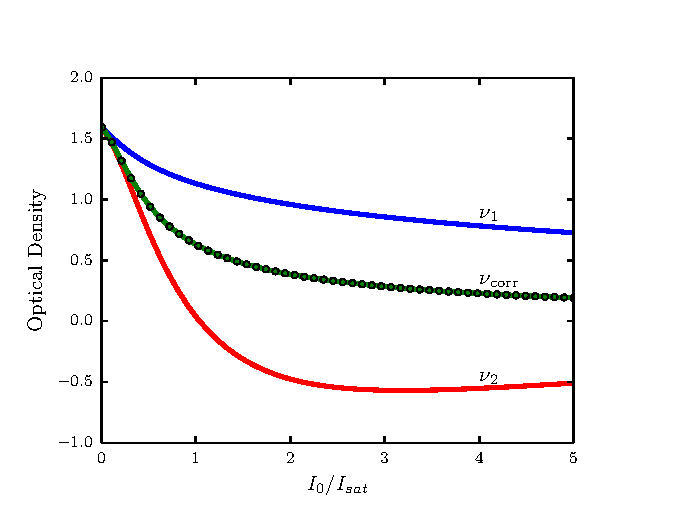
\includegraphics{figure7.pdf}}
	\subfigure[]{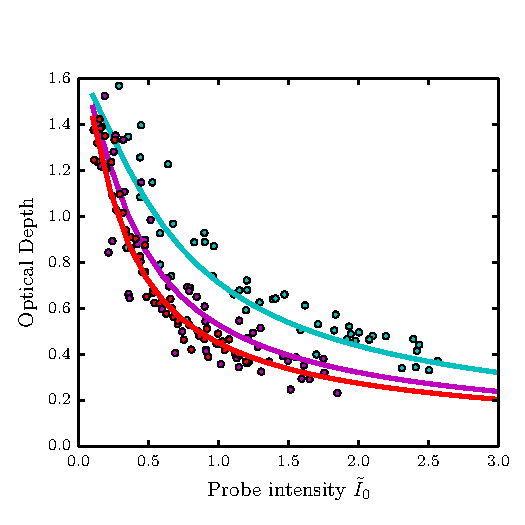
\includegraphics{figure8.pdf}}
\caption{(a) Top. Optical depth as a function of probe intensity for an imaging time $t=100$ \us. $OD^{\rm{(1)}}$ and $OD^{\rm{(2)}}$ are optical depths predicted from a given column density by Eq. (\ref{eq2}) and (\ref{eq:OD2}) respectively.  The two versions of simulated optical depth, $OD^{\rm{sim1}}$ (green curve) and $OD^{\rm{sim2}}$ (green dots) are plotted. Bottom. The fractional difference between two versions of the simulated $OD$, $\left|OD^{\rm{sim1}}-OD^{\rm{sim2}}\right|/OD^{\rm{sim1}}$. (b) The optical depth as a function of probe intensity for three imaging times: $t=40$ \us{} (cyan),  $t=75$ \us{} (magenta),  $t=100$ \us{} (red). The dots represent experimental data and the lines represent the best fit of simulated data. The optimal fit parameters pictured are a $\sigma_0 n$ of 1.627(5) and saturation intensity of 29(7) counts/\us{}.  }
\label{fig:compareModelsAndIsat}
\end{figure}

\subsection{SNR optimization}
This simulation allowed us to interpret experimental data. For a given imaging time, we created a look-up table of predicted optical depth as a function of probe intensity and atomic column density. We then found the observed optical depth on this table, with the given probe intensity, and inferred the atomic density. The uncertainty in the measured intensities can be propagated through this procedure, and we established optimal imaging parameters to maximize the SNR of this detection scheme.
\par The only source of measurement uncertainty we considered was the Poisson noise on the detected arriving photons (i.e., photoelectrons) with standard deviation proportional to $q_{\rm{e}}\sqrt{N_p}$, where $q_{\rm{e}}$ is the quantum efficiency of the camera and $N_p$ is the photon number. We then propagated this uncertainty through our correction scheme to obtain the uncertainty in our deduced value of $\sigma_0 n$. We define the SNR as $\sigma_0 n/\delta_{\sigma_0 n}$, where $ \delta_{\sigma_0 n}$ is the propagated measurement uncertainty.
\par As seen in Fig. \ref{fig:SNR}(a), after about 40 \us{} extending the imaging time no longer yields appreciable improvement in SNR. Imaging for 40 \us{} as opposed to 10 \us{} where the uncorrected model is appropriate, improves the SNR by a factor of  1.5. We performed the experiments described in the second section at 40 \us{} imaging time. Figure \ref{fig:SNR}(b) shows that the optimal probe intensity varies with the atomic column density. For low atom numbers, $\sigma_0 n\approx0.1$, a probe intensity of $\tilde{I}_0\approx0.6$ is best. However, in our experiment the probe intensity had a Gaussian profile and was not uniform over the whole image.  The typical probe intensities used in our experiments varied over the $2\tilde{I}_0=0.1-0.7$  range.
\begin{figure}
	\subfigure[]{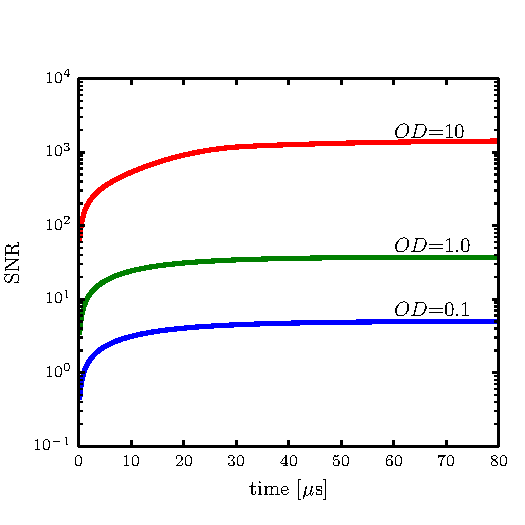
\includegraphics{figure9a.pdf}}
	\subfigure[]{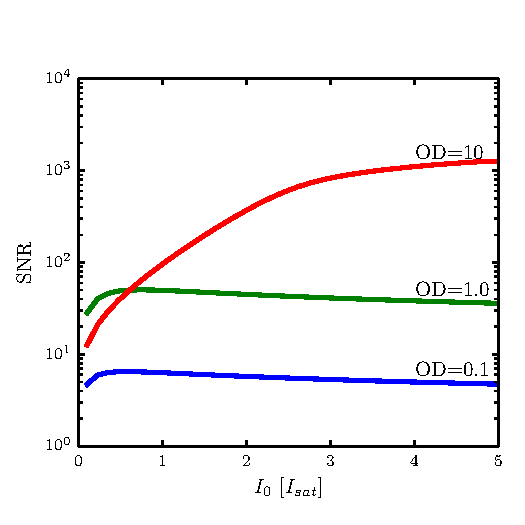
\includegraphics{figure9b.pdf}}
\caption{SNR for three different column densities after correcting for recoil induced detuning. (a) SNR as a function of imaging time for a probe intensity of $\tilde{I}_0=5.0$ and (b) SNR as a function of probe intensity for an imaging time of 50 \us{}.}
\label{fig:SNR}
\end{figure}

\subsection{Calibration of saturation intensity}
Our absorption images were taking using a charge-coupled device (CCD) camera.  Each camera pixel  converted the photons it was exposed to, with some efficiency, into photoelectrons, and digitally returned an integer, called `counts', that was proportional to the radiant fluence.  However, the proportionality constant depends on many factors, such as the quantum efficiency of the camera, the electronic gain during the readout process, losses in the imaging system and the polarization of the probe light.
\par We determined this proportionality constant through direct measurement. In the limit where the system is adequately described by $\sigma_0 n=-\ln(\tilde{I}_f/\tilde{I}_0)$, only the ratio of the initial and final intensities matter, and this proportionality constant is irrelevant. In all other regimes, however, the ratio of the initial and final intensities to the saturation intensity also comes into play, making the proportionality constant significant. One way to approach this calibration is to determine the saturation intensity in units of `counts' per unit time.
\par To calibrate the saturation intensity in camera counts per unit time, we took absorption images of \K{} clouds at three different imaging times (40 \us{}, 100 \us{}, and 200 \us{}) with varying probe intensities. In a small region at the center of the cloud the atomic density was approximately uniform, and we averaged the initial and final intensities of each pixel in that region. Thus, for each image we obtained $\tilde{I}_0$ and $\tilde{I}_f$, in counts per microsecond. We then simultaneously fit our simulated optical depth  $OD^{\rm{sim}}$ to this full data set, with the atomic density $\sigma_0 n$ and  $I_{\rm{sat}}$ in counts per microsecond as free parameters. As seen in Fig. \ref{fig:compareModelsAndIsat}(b), the model produced a good fit to the experimental data, and provided a calibration of the saturation intensity for our experiment.
%\begin{figure}
%	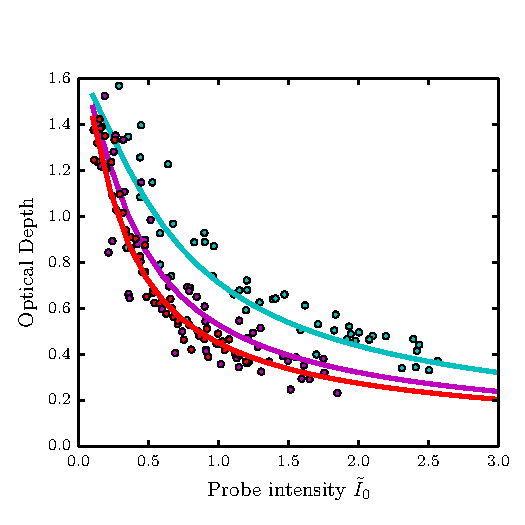
\includegraphics{figure8.pdf}
%\caption{The optical depth as a function of probe intensity for three imaging times: $t=40$\us{} (blue),  $t=75$\us{} (green),  $t=100$\us{} (red). The dots represent experimental data and the lines represent the best fit of simulated data. The optimal fit parameters pictured are a $\sigma_0 n$ of 1.62 and saturation intensity of 29 counts/\us{}. }
%\label{fig:isatCalib}
%\end{figure}


\section{\swave{} scattering experiment}
In this section we describe our Fermi scattering experiment. We collided two counter-propagating \K{} clouds and observed the resulting \swave{} halo of scattered atoms.  We measured the dependence of the scattered atomic fraction on the bias magnetic field in the vicinity of the Feshbach resonance. We used this data to extract the location of the magnetic fields resonance of 20.206(15) \mT{} and a width of 1.0(5) \mT{}, similar to the accepted values of 20.210(7) \mT{} and 0.78(6) \mT{} \cite{Regal04}.
\subsection{Experimental procedure}
We prepared clouds of cold \K{} atoms in a hybrid \K{} and \Rb{} apparatus, previously described in \cite{Williams13, Lin09, KarinaThesis}. We used a Zeeman slower to slow both species before capturing in a magneto-optical trap (MOT). After 7 s seconds of MOT loading \K{} followed by 1.5 s of loading both \K{} and \Rb{}, we cooled both species in optical molasses for 2 ms. We optically pumped both species into their maximally stretched magnetically trappable states, $\ket{F=9/2, m_F=9/2}$ for \K{} and $\ket{F=2,m_F=2}$ for \Rb{}. Both species were then loaded into a quadrupole magnetic trap with a $\approx$ 7.68 mT/cm gradient along \ez{}, and cooled evaporatively via forced RF evaporation, sweeping the RF frequency from 18 MHz to 2 MHz in 10 s. The magnetic trap was plugged by a $\lambda =$ 532 nm beam, tightly focused to $\approx$ 30 \um{} and $\approx$ 5 W in power, providing a repulsive potential around the zero field point to prevent Majorana losses. Since the \K{} atoms were spin polarized and therefore only interacted by the strongly suppressed \pwave{} interactions, they re-thermalized only due to sympathetic cooling with \Rb{} atoms.

We then loaded the atoms into a crossed optical dipole trap, provided by a 1064 nm fiber laser, and continued evaporative cooling by slowly ramping down the dipole trap to trap frequencies of $(\omega_x,\omega_y,\omega_z)/2\pi =(39, 42, 124)$ Hz in the three spatial directions, while also turning off the quadrupole field. We then used adiabatic rapid passage (ARP) to transfer the \Rb{} atoms from the $\ket{F=2, m_F=2}$ state to the  $\ket{F=1, m_F=-1}$ absolute ground state via 6.8556 GHz microwave coupling (20.02 MHz from the zero field resonance) followed by a magnetic field sweep from -0.469 mT to -0.486 mT in 50 ms. This state was chosen to minimize spin changing collisions with \K{} atoms during any further evaporation \cite{BestThesis}.  We then briefly applied an on-resonant probe laser, ejecting any remaining \Rb{} atoms in the $F=2$ manifold from the trap. We again used ARP to transfer the \K{} atoms into the $\ket{F=9/2,m_F=-9/2}$ state by using a 3.3 MHz rf field and sweeping the bias magnetic field from -0.518 mT to -0.601 mT in 150 ms.

Following the state transfer, we had two versions of the protocol \--- one for approaching the Feshbach resonance from higher fields and one for approaching it from lower fields. For approaching the resonance from lower fields, we proceeded by ramping the bias magnetic field to 19.05 mT, turning on a 42.42 MHz RF field, and then sinusoidally modulating the bias field at 125 Hz for 0.5 s, with a 0.14 mT amplitude, decohering the \K{} state into an equal mixture of $\ket{F=9/2,m_F=-9/2}$ and $\ket{F=9/2,m_F=-7/2}$. For approaching the resonance from higher fields, the same was done at a bias field of 21.71 mT and an RF frequency of 112.3 MHz. The depolarization allowed the \K{} atoms to interact and re-thermalize, allowing us to further evaporate in the dipole trap \cite{DeMarco99}. Since \Rb{} is heavier than \K{}, we were able to evaporate the \K{} atoms past the point where \Rb{} atoms were no longer suspended against gravity and had been completely removed.  These hyperfine states of \K{} were then used to study their Feshbach resonance.
\par After evaporation, we ramped the bias field in a two-step fashion to the desired value $B$ near the Feshbach resonance. We approached the field using a large pair of  coils in Helmholtz configuration (0.19 mT/A) to bring the magnetic field to a setpoint 0.59 \mT{} away from $B$,  $B-0.59$ \mT{} when approaching from below and $B+0.59$  \mT{} from above. We held the atoms at this field for 100 $\rm{ms}$ to allow the eddy currents induced by the large coils to settle, and then used a lower inductance (0.017 mT/A) set of Helmholtz coils to quickly change the field the remaining 0.59 \mT{}. This allowed us to study the resonance from both sides without the added losses associated with going through the resonance \cite{Chin10}.

Once at the intended bias field, we split the cloud into two spatially overlapping components with opposing momenta  and observed scattering as they moved through each other and separated. These counterpropagating components were created using an  8$E_{\rm{L}}$ deep near resonant ($\lambda_{\rm{L}}$=766.704 nm) 1-d retro-reflected optical lattice, where $E_{\rm{L}}=\hbar^2 k_{\rm{L}}^2/2m_{\rm{K}}$ is the lattice recoil energy and $\hbar k_{\rm{L}}=2\pi \hbar/ \lambda$ is the recoil momentum. We rapidly pulsed this lattice on and off with a double-pulse protocol \cite{Wu05, Edwards10}. The pulse sequence was optimized to transfer most of the atoms into the $\pm 2 \hbar k_{\rm{L}}$ momentum states. Since the initial Fermi gas had a wide momentum spread (in contrast to a BEC, which has a very narrow momentum spread), and the lattice pulsing is a momentum dependent process  \cite{Wu05}, not all the atoms were transferred into the target momentum states. We optimized our pulse times to minimize the atoms remaining in the zero momentum state. The optimized pulse times were 23 \us{} for the first pulse, 13 \us{} off interval, and 12 \us{} for the second pulse \cite{Edwards10}.

We then released the atoms from the trap and allowed 1 ms for the two opposite momentum states within the cloud to pass through each other, scattering on the way. For the data taken coming from below the Feshbach resonance, we then simply ramped down the field and imaged the atoms. For the data taken coming from above the Feshbach resonance, we ramped the field back up, retreating through the resonance if it had been crossed and thereby dissociating any molecules that were created, and then quickly ramped the field back down and imaged the atoms. We used a 40 \us{} imaging pulse with $I_0/I_{\rm{sat}}\approx 0.6$ at the center of the probe laser.

The total time-of-flight, the time from the moment the atoms were released from the trap to when they were imaged, was $t_{TOF}=6.8$ $\rm{ms}$. In such an image, the observed atomic position is determined by the initial velocity upon release from the trap, along with the time-of-fligt time $t_{TOF}$. Therefore, this technique measures the momentum and not the position distribution of the atoms.

The magnetic fields produced by our coils in the regime of interest were independently calibrated by rf-spectroscopy. We prepared \K{} atoms in the $\ket{F=9/2, m_F=-9/2}$ state and illuminated them with and rf-field with some frequency $\nu_{rf}$. We then ramped our high-inductance coils to variable set points, followed by an adiabatic 250\us{} ramp of 2.84 mT in the lower inductance coils. We then used Stern-Gerlach and observed the fractional population in the $\ket{F=9/2, m_F=-9/2}$  and $\ket{F=9/2, m_F=-7/2}$ states as a function of the high-inductance coil current. We fit the fractional population curve to a Gaussian, and considered the center of the fit to be on-resonant, with an uncertainty given by the Gaussian width. We used the Breit-Rabi formula to determine the resonant field value at $\nu_{rf}$. We did this for 5 different rf frequencies, and acquired a field calibration with an uncertainty of 0.3 mT, which was included in the listed uncertainty on the center field of the Feshbach resonance.


\subsection{Methods}

We first processed each image by comparing the obsereved $OD$s to simulations taking into account the recoil induced detuning as described in Sec. \ref{sec:2}. An example of images before and after processing are shown in Fig. \ref{fig:SampleCorrection}.  To improve the signal and mitigate our shot to shot number fluctuations, we took 15 nominally identical images for each data point.
\begin{figure}
	\subfigure[]{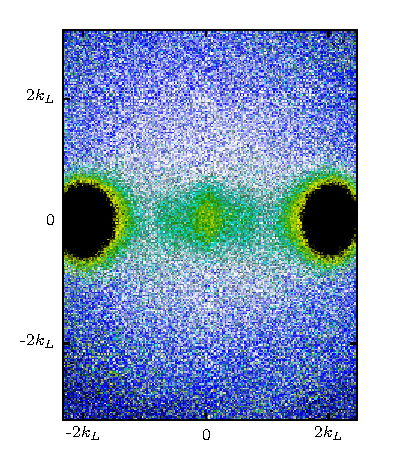
\includegraphics{figure10a.pdf}}
	\subfigure[]{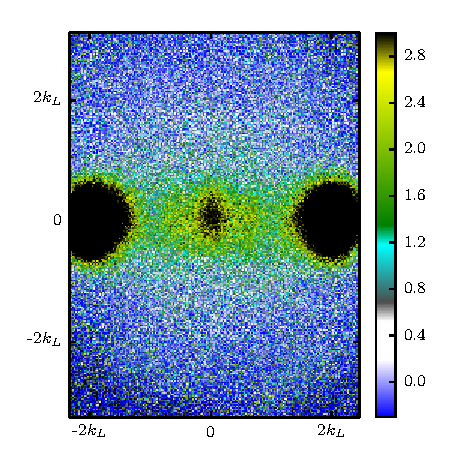
\includegraphics{figure10b.pdf}}
\caption{An example of our absorption image after 6.8 ms TOF. The 1-D lattice imparts momentum along \ex{}. The two large clouds on the left and right are the atoms in the $\pm 2 k_{\rm{L}}$ momentum orders that passed through each other unscattered. The smaller cloud in the center is the atoms that remained in the lowest band of the lattice after pulsing, and thus obtained no momentum. The thin spread of atoms around these clouds is the atoms that underwent scattering.   This image was taken coming from below the Feshbach resonance at 20.07  \mT{}. (a) Raw optical depth, (b) atomic column density obtained by comparing to simulated $OD$s, $\sigma_0 n^{\rm{sim}}$ }
\label{fig:SampleCorrection}
\end{figure}

We counted the fraction of atoms that experienced a single scattering event for each of the fifteen images at a given bias magnetic field. Single scattering events are easily identified, as two atoms that scatter elastically keep the same amplitude of momentum, but depart along an arbitrary direction. Therefore, an atom traveling at $2 \hbar k_{\rm{L}}$ to the right that collides elastically with an atom traveling at $-2 \hbar k_{\rm{L}}$ to the left will depart with equal and opposite momenta $2 \hbar k_{\rm{L}}$ at an arbitrary angle, and in a time of flight image such atoms will lie in a spherical shell, producing the scattering halo pictured in Fig. \ref{fig:halo}(a).
\begin{figure}
	\subfigure[]{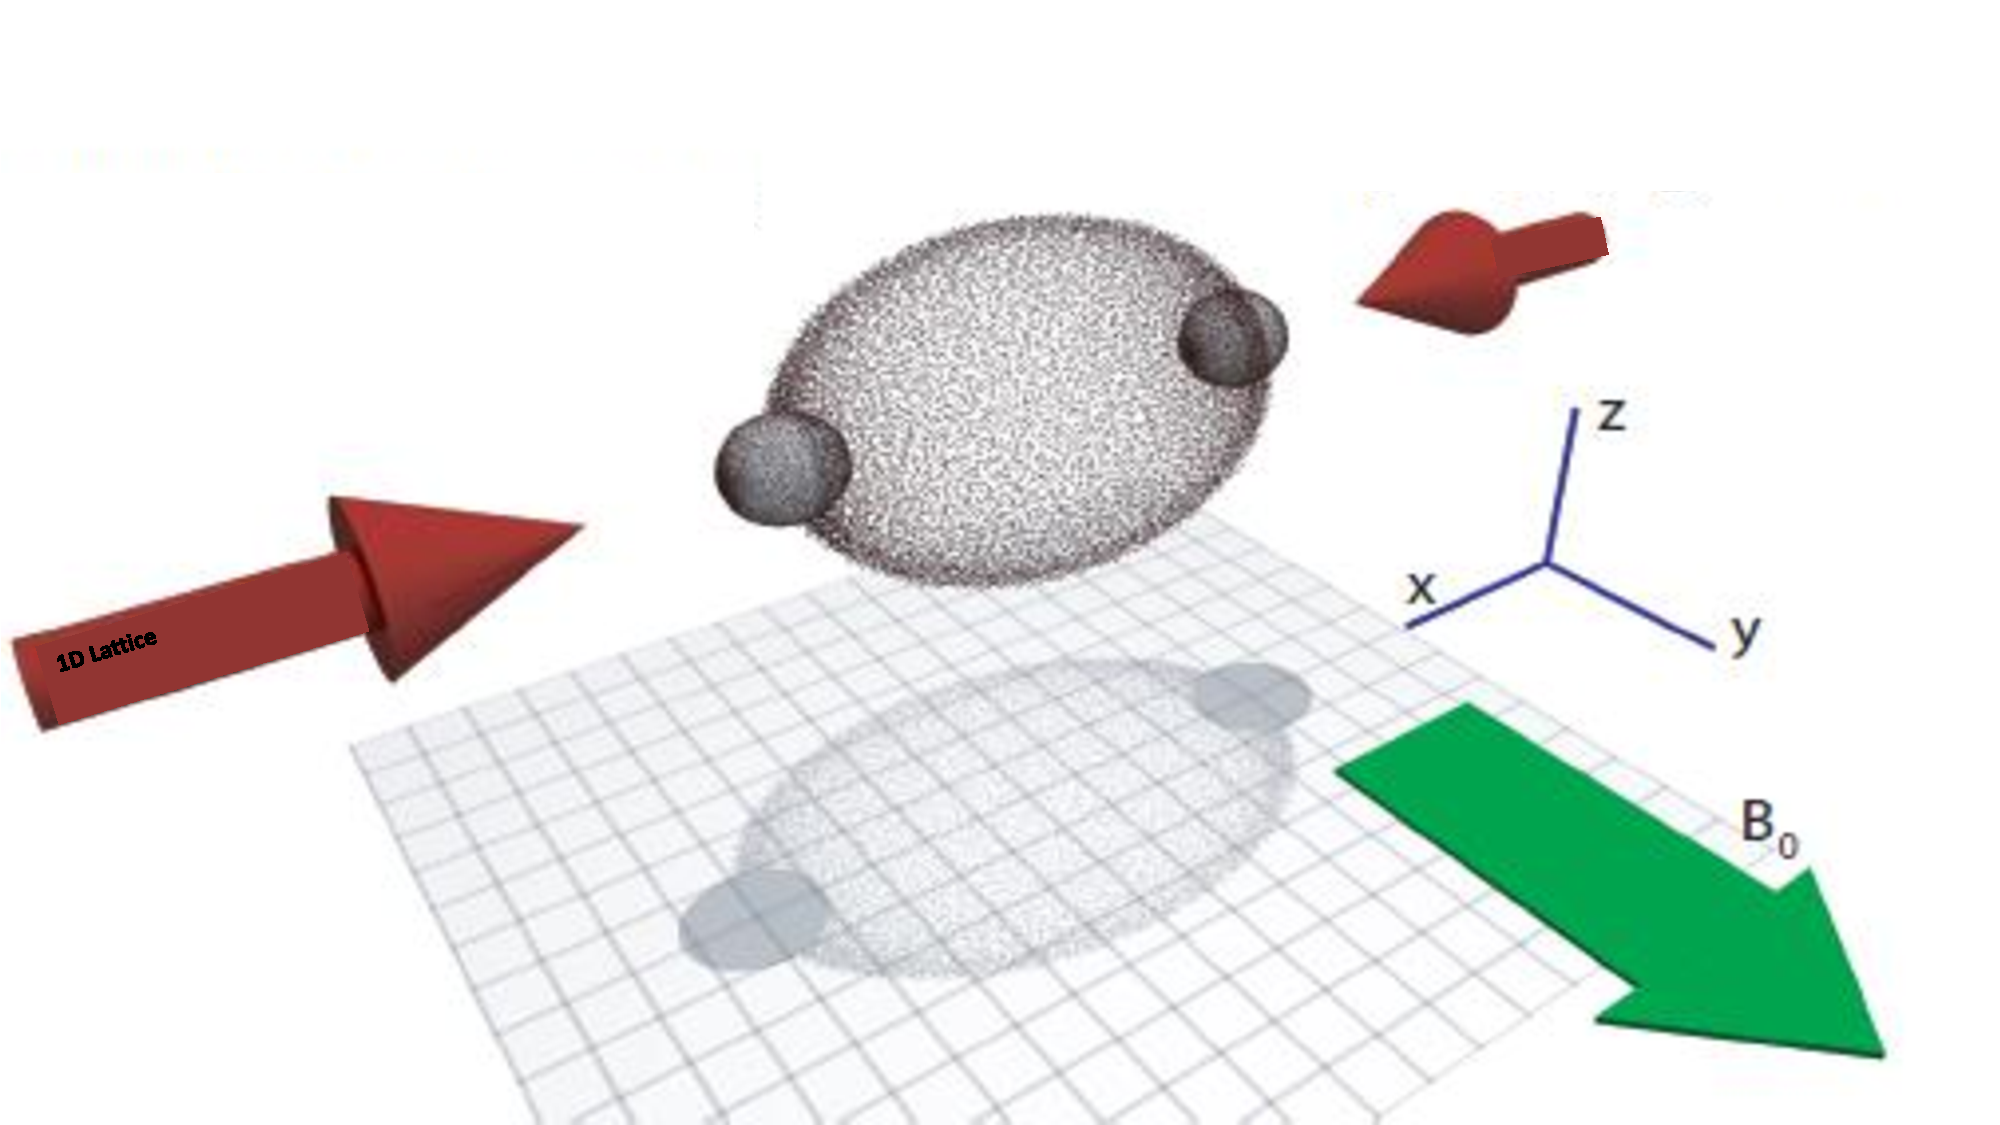
\includegraphics[scale=0.25]{Picture12.pdf}}
	\subfigure[]{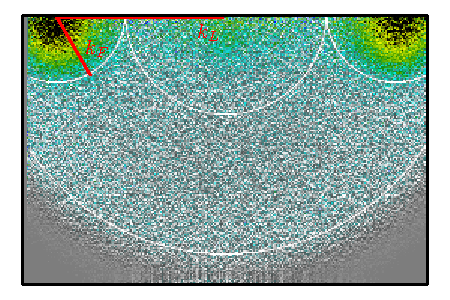
\includegraphics{figure12b.pdf}}
\caption{(a) Our experimental setup. After time of flight, the two clouds traveling along $\pm \hat{e}_x$ directions have separated and the atoms that underwent a single scattering event were evenly distributed in a scattering halo around the unscattered clouds. The 1-D lattice defined the axis of cylindrical symmetry. (b) Inverse Abel transformed image. The atoms within the Fermi momentum $k_F$ of each unscattered cloud center are in the unscattered region and counted towards the total unscattered number. The atoms outside the radius $ k_{\rm{L}}-k_{\rm{F}}$ but inside $k_{\rm{L}}+k_{\rm{F}}$ but outside the unscattered region are counted towards the number of single scattered atoms.   }
\label{fig:halo}
\end{figure}

Absorption images captured the integrated column density along \ez{}, a projected 2D atomic distribution. To extract the radial dependence of the 3D distribution from the 2D image, we performed a standard inverse Abel transform. The inverse Abel transform assumes cylindrical symmetry, which was present in our case, with the axis of symmetry along \ex{}, defined by the lattice. We neglect the initial asymmetry of the trap, as during time-of-flight the atoms travel far beyond the initial extent of the cloud  $(r_x,r_y,r_z)\approx$ (45,48,15) \um{}, while the cloud width after TOF is $\approx$ 82 \um in each direction. We thus obtained the atomic distribution $\rho(r,\theta)$ as a function of $r$, the radial distance from the scattering center, and $\theta$, the angle between $r$ and symmetry axis \ex{}, integrated over $\phi$, the azimuthal angle around the $x$ axis.

We then extracted the number of scattered atoms $N_{\rm{scat}}$ as a fraction of the total atom number $N_{\rm{tot}}$ for each image, as shown in Fig. \ref{fig:halo}(b). The unscattered atom number was the number of atoms in the two unscattered clouds. The number of atoms that underwent a single scattering event was the number of atoms outside the Fermi radius of the unscattered clouds, but inside the arc created by rotating the Fermi momentum $k_{\rm{F}}$ around the original center of the cloud (red arcs in Fig. \ref{fig:halo}(b)). For both the scattered and unscattered numbers, we accounted for atoms that fell outside the field of view of our camera by multiplying the counted atom number by a factor of the total area as defined by the radii divided by the visible area on the camera. The atoms in the center region were not counted as they were originally in the zero momentum state and could not contribute to the scattering halo under study.

We fit the fraction of scattered atoms versus the total atom number for each of the 15 images taken at the same bias magnetic field to a line constrained to be zero at zero. The slope of this fit was taken to be the value of $N_{\rm{scat}}/N_{\rm{tot}}^2$ at that bias magnetic field, and the variance of the fit gave the uncertainty on that data point. This uncertainty reflected our shot to shot number fluctuations, which produced variable atomic densities and thus influence the scattered fraction. 

We then deduced the resonant field value $B_0$ and width of the resonance  $\Delta$, the parameters in Eq. (\ref{feshbachEq}).  Since we were in the low energy regime (the atomic momentum was much smaller than the momentum set by the van der Waals length $k_{\rm{L}}+k_{\rm{F}}\ll1/l_{\rm{vdW}}$, and we were well below the p-wave threshold temperature \cite{DeMarco99}), the scattering cross-section was given by $\sigma=4\pi a^2$.

The scattering cross-section $\sigma$ gives the probability $P_{\rm{scat}}=\sigma N/A$ that a single particle will scatter when incident on a cloud of atoms with a surface density of $N/A$, where $A$ is the cross-sectional area of the cloud and $N$ is the number of atoms in the cloud. In our case, each half of the initial cloud, with atoms number $N_{\rm{tot}}/2$, is incident on the other half. Thus, the number of expected scattering events is $N_{\rm{scat}}= (N_{\rm{tot}}/2) \sigma  (N_{\rm{tot}}/2)=\sigma N_{\rm{tot}}^2/4A$. Assuming $A$ is constant for all our data, we can define a fit parameter $b_0=4\pi a_{\rm{bg}}^2/4A$, where $a_{\rm{bg}}$ is the background scattering length. We can thus adapt Eq. (\ref{feshbachEq}) to obtain the fit function
\begin{equation}
\frac{N_{\rm{scat}}}{N_{\rm{tot}}^2}=b_0\left(1-\frac{\Delta}{B-B_0}\right)^2 + C.
\label{eq:fit}
\end{equation}
We found that our imaging noise skewed towards the positive, giving rise to a small background offset. We accounted for this in our fit by including a constant offset parameter $C$.


\subsection{Results}
Our final data is presented in Fig. \ref{fig:fittedFractions}. The red curve depicts a best fit of the model given in Eq. (\ref{eq:fit}). The fit parameters we extracted were $\Delta = 1(5)$  \mT{}, $B_0 = 20.206(15)$  \mT{}, $b_0 = 5(3)\times 10^{-3}$ and $C=8(1)\times 10^{-4}$. To obtain the fit, we used data taken by approaching the resonance from above for points above where we expected the resonance to be and data taken approaching the resonance from below for points below. We also excluded from the fit data points very near the resonance, as there the assumption $\sigma\rho\ll1$, where $\rho$ is the atom number per unit area, is no longer valid and the problem must be treated hydrodynamically.

The accepted values for the $^{40}K$ s-wave Feshbach resonance for the  $\ket{9/2,-9/2}$ and $\ket{9/2,-7/2}$ states are $B_0=20.210(7)$  \mT{} and $\Delta=0.78(6)$  \mT{} \cite{Regal04}, which is in good agreement with our findings. Some potential sources of systematic uncertainty that we did not account for include scattering with atoms that did not receive a momentum kick from the lattice pulsing or the impact of multiple scattering events.
\begin{figure}
	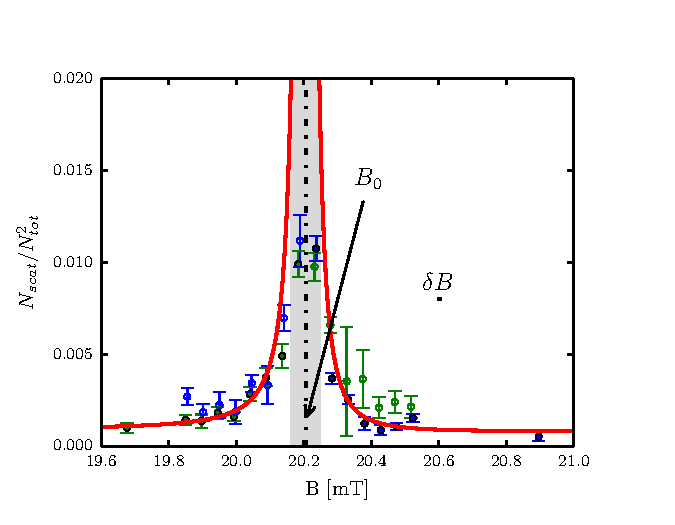
\includegraphics{figure11.pdf}
\caption{Normalized scattered population plotted versus bias field $B$. Green dots represent data taken coming from below the resonance, and blue dots represent the data taken coming from above the resonance. The red curve depicts the best fit, where data coming from above the resonance was used above the resonance and data coming from below the resonance was used below the resonance to create the fit; the unused data points are indicated by hollow dots. The regime where the scattering length is likely large enough for the atoms to behave hydrodynamically is shaded in gray, and data points in that area were also excluded from the fit. Resonant field value $B_0$ as found in this work and our systematic uncertainty in the bias magnetic field $\delta B_0$ are indicated.    }
\label{fig:fittedFractions}
\end{figure}
\section{Conclusion}
We studied the effects of recoil-induced detuning effects on absorption images and found an optimal imaging time of $\approx40$ \us{} for \K{} atoms for noise minimization after corrections. We use these results to observe s-wave scattering halos of the Fermi gas around the $\approx 20.2$ \mT{} Feshbach resonance and directly verified the resonance location and width. Our analysis can be used in any absorption imaging application where SNR optimization is critical.
\section*{Acknowledgments}
We thank Marcell Gall for helpful discussions. This work was partially supported by the ARO’s Atomtronics MURI, by the
AFOSR’s Quantum Matter MURI, NIST, and the NSF through the PFC at the JQI. B.K.S. is
a NIST-NRC Postdoctoral Research Associate. L.M.A. was supported by the NSF GRFP.

\section*{References}
\bibliography{refs}{}
\bibliographystyle{unsrt}

\end{document}

